% !TeX spellcheck = en_GB
\documentclass[11pt]{exam}
% addpoints,

\usepackage[type1]{libertine}
\usepackage[a4paper]{geometry}
\usepackage{amsmath, amsthm, amssymb} 
\usepackage{parskip}
\usepackage{tabularx}
\usepackage[english]{babel}
\usepackage{enumitem}
\usepackage{gensymb}
\usepackage{bm}
\usepackage{graphicx}
\usepackage{xcolor}
\usepackage{float}
\usepackage{wrapfig}
\usepackage{cancel}
\usepackage{multicol}
\usepackage{commath} % Provides good differentials
\usepackage{siunitx} % Provides good units
\usepackage{nicefrac}

\usepackage[titletoc,title,toc,page]{appendix}
\usepackage{hyperref}
\hypersetup{
	pdftitle={Dynamics Problem Set},
	pdfauthor={Sun Yudong},
	bookmarksnumbered=true,
	bookmarksopen=true,
	bookmarksopenlevel=2,
	pdfstartview=Fit,
	pdfpagemode=UseOutlines,
	colorlinks=true,
	linkcolor=black,
	filecolor=magenta,      
	urlcolor=blue
}

\newenvironment{multicolFigure}
{\par\medskip\noindent\minipage{\linewidth}}
{\endminipage\par\medskip}
% https://tex.stackexchange.com/questions/12262/multicol-and-figures

%\newenvironment{amatrix}[1]{%
%	\left(\begin{array}{@{}*{#1}{c} | c@{}}
%	}{%
%	\end{array}\right)
%}						% https://tex.stackexchange.com/a/2238
%\usepackage{blkarray}	% https://tex.stackexchange.com/a/59519
%\usepackage{mathtools}	% https://tex.stackexchange.com/a/103993

\title{Dynamics Problem Set\\ {\large involving Forces, Momentum and WEP}}
\author{Sun Yudong}
\date{April 1, 2018}

\begin{document}
	\maketitle
	\begin{questions}
		\setlength\itemsep{0.2\baselineskip}        % https://tex.stackexchange.com/a/140037
		\question{
			A small car collides head-on with a large SUV. Which of the following statements concering this collision are correct? (There may be more than one correct choice)
			\begin{choices}
				\choice{Both vehicles are acted upon by the same magnitude of average force during the collision.}
				\choice{The small car is acted upon by a greater magnitude of average force than the SUV.}
				\choice{The small car undergoes a greater change in momentum than the SUV}
				\choice{Both vehicles undergo the same change in magnitude of momentum}
			\end{choices}
			\begin{solution} A and D \end{solution}
		}
		\vfill
		\question{
			A ball of mass \SI{0.18}{\kilogram} moving with speed \SI{11.3}{\meter\per\second} collides head-on with an identical stationary ball. (Notice how we do not know the type of collision.) Which of the following quantities can be calculated from this information alone?
			\begin{choices}
				\choice{The force each ball exerts on the other.}
				\choice{The velocity of each ball after the collision.}
				\choice{Total kinetic energy of both balls after the collision.}
				\choice{Total momentum of both balls after the collision.}
			\end{choices}
			\begin{solution} D \end{solution}
		}
		\vfill
		
		\ifprintanswers
			\pagebreak
		\fi
		
		\question{
			You drop an egg from rest with no air resistance. As the egg falls, 
			\begin{choices}
				\choice{only its momentum is conserved.}
				\choice{only its kinetic energy is conserved.}
				\choice{both its momentum and its mechanical energy are conserved.}
				\choice{its mechanical energy is conserved, but its momentum is not conserved.}
			\end{choices}
			\begin{solution}D. Do note that, however, if we consider the entire system of the egg and the Earth (and the air), momentum is still conserved. \end{solution}
		}
	
		\ifprintanswers
			\vfill
		\fi

		\question{
			You, at \SI{70.0}{\kilogram}, are standing stationary on a sheet of ice that covers the football stadium parking lot in Buffalo; there is negligible friction between your feet and the ice. A \SI{50.0}{\kilogram} friend throws you a \SI{0.400}{\kilogram} ball.
			\begin{parts}
				\part If your friend moves back at a speed of \SI{0.0800}{\meter\per\second}, what is the speed of the ball?
				\begin{solution}
					\begin{equation*}
					v_b = \frac{50.0 \times 0.0800}{0.400} = \frac{4}{0.4} = \SI{10.0}{\meter\per\second}
					\end{equation*}
				\end{solution}
			
				\part If you catch the ball, with what speed do you and the ball move afterwards?
				\begin{solution}
					\begin{equation*}
					v_{combined} = \frac{4}{0.400 + 70.0} = \SI{5.68e-2}{\meter\per\second}
					\end{equation*}
				\end{solution}
			
				\part If the ball hits you and bounces off your chest, so that afterwards it is moving horizontally at \SI{8.00}{\meter\per\second} in the opposite direction, what is your speed after the collision?
				\begin{solution}
					\vspace{-0.5cm}
					\begin{align*}
					m_{ball}u_{ball} &= m_{ball}v_{ball} + m_{you}v_{you} \\
					v_{you} &= \frac{m_{ball}\left(u_{ball} - v_{ball}\right)}{m_{you}} \\
					&= \frac{0.400\left[10.0 - \left(-8.00\right)\right]}{70.0} \\
					&= \SI{1.03e-1}{\meter\per\second}
					\end{align*}
					\vspace{-0.5cm}
				\end{solution}
			\end{parts}
		}
		\vfill
		\question{
			\textbf{[Poorly Maintained Car]} John was driving his \SI{1.50e3}{\kilogram} car up a hill when the engine suddenly dies and the gear disengages, causing his vehicle to free-wheel\footnote{The wheels are no longer driven by the engine}. Having missed his car servicing for many years, his brakes were also faulty. Hoping to stay alive, he jumps out of the car as his car slows to a momentary stop along the hill at $h = \SI{100}{\meter}$ above sea level. As he turns around, he sees his car roll down the hill and crash into a \SI{5.00e3}{\kilogram} truck parked at the bottom of the hill. 
			
			You may disregard any resistive forces in the wheels.
			
			\begin{parts}
				\part If the car and truck fuse together, at what speed would the car/truck combination be moving?
				\begin{solution}
					\vspace{-0.5cm}
					\begin{align*}
						\text{GPE} = \cancel{m}gh &= \frac{1}{2} \cancel{m}v_i^2 = \text{KE} \\
						v_i &= \sqrt{2gh} \\
						P_i = mv_i = m\sqrt{2gh} &= (m+M)v_f = P_f \\
						v_f &= \frac{m\sqrt{2gh}}{m+M} = \SI{10.2}{\meter\per\second}
					\end{align*}
					\vspace{-0.5cm}
				\end{solution}
				\part The car/truck combination then slides without slowing into an abandoned building at the end of the road and crashes into a rigid wall. What is the average force of the rigid wall on the car/truck combination, if the entire collision happens in \SI{0.8}{\second}?
				\begin{solution}
					\vspace{-0.5cm}
					\begin{align*}
						F = \frac{\Delta P}{\Delta t} &= \frac{m\sqrt{2gh}}{\Delta t} \\
						&= \SI{8.31e4}{\newton}
					\end{align*}
					\vspace{-0.5cm}
				\end{solution}
			\end{parts}
		}
		\vfill
		
		\ifprintanswers
			\pagebreak
		\fi
		
		\question{
			A \SI{15.0}{\kilogram} block is attached to a very light horizontal spring of force constant \SI{500}{\newton\per\meter} and is resting on a frictionless horizontal table. Suddenly it is struck by a \SI{3.00}{\kilogram} stone travelling horizontally at \SI{8.00}{\meter\per\second} to the right, whereupon the stone rebounds at \SI{2.00}{\meter\per\second} horizontally to the left. Find the maximum distance that the block will compress the spring after the collision. (\textit{Hint:} Break this problem into two parts --- the collision and the behaviour after the collision --- and apply the appropriate conservation law to each part.)
			
			\begin{figure}[h]
				\centering
				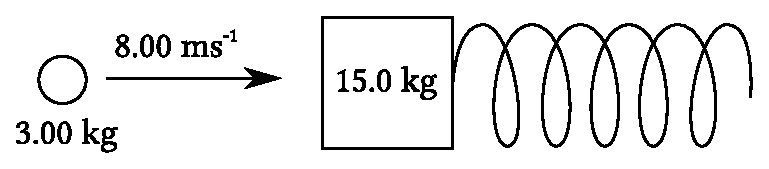
\includegraphics[width=7cm]{springmomentum.eps}
			\end{figure}
		
			\begin{solution}
				We define right as positive. At the moment of collision,
				\begin{align*}
				P_i &= P_f \\
				m_{stone}u_{stone} &= m_{stone}v_{stone} + m_{block}v_{block} \\
				v_{block} &= \frac{m_{stone}\left(u_{stone} - v_{stone}\right)}{m_{block}} = \frac{3.00(8 + 2)}{15} \\
				&= \SI{2.00}{\meter\per\second} 
				\end{align*}
				After the collision, the KE imparted on the \SI{15.0}{\kilogram} block is all converted to EPE.
				\begin{align*}
				\text{KE} &= \text{EPE} \\
				\cancel{\frac{1}{2}}m_{block}v_{block}^2 &= \cancel{\frac{1}{2}}kx_{max}^2 \\
				x_{max} &= \sqrt{\frac{m_{block}v_{block}^2}{k}} \\
				&= \sqrt{\frac{15.0 \times 2.00^2}{500}} \\
				&= \frac{\sqrt{3}}{5} \SI{}{\meter}
				\end{align*}
				\vspace{-0.5cm}
			\end{solution}
		}
		\vfill
		
		\pagebreak

		\question{\textbf{[A Cart of Sand]} Consider a cart full of sand with total mass of $M$ moving at a constant velocity $v$ on a frictionless track.
			\begin{parts}
				\part A crack forms at the bottom of the cart and sand is leaking out at a rate of $\dif m/\dif t=\sigma$. What will the velocity of the cart be?
				\begin{solution}$v$\end{solution}
				\part If you apply a force $F$ to the leaking cart, what is its acceleration?
				\begin{solution}$\displaystyle a = \frac{F}{M - \sigma t}$\end{solution}
				\part The sand then falls (vertically) into a passing cart travelling at $2v$ below the tracks. With what force must you push on the cart to keep it moving (horizontally) at a constant speed $2v$?
				\begin{solution}$\displaystyle F = \dod{p}{t} = ma + \dod{m}{t}v = 0 + \sigma v$\end{solution}
			\end{parts}
		}
	\end{questions}

	\ifprintanswers
		% \pagebreak
	\else
		\vfill
	\fi
	\section*{Challenging Questions}
	\begin{questions}
		\question{
			\textbf{[Walking in a boat]} A \SI{45.0}{\kilogram} woman stands up in a \SI{60.0}{\kilogram} canoe of length \SI{5.00}{\meter}. She walks from a point \SI{1.00}{meter} from one end to a point \SI{1.00}{meter} from the other end. If the resistance of the water is negligible, how far does the canoe move during the process?
			
			\begin{figure}[h]
				\centering
				\includegraphics[width=10cm]{canoe.png}
			\end{figure}
			\ifprintanswers
				\pagebreak
			\fi
			\begin{solution}
				Suppose the woman moves at some point with some velocity $v_w$ to the right \underline{relative to the stationary river bank}. We define right as positive. By conservation of momentum, we know that:
				\begin{align*}
					m_wv_w + m_cv_c &= 0\\
					v_c &= -\frac{m_w}{m_c}v_w
				\end{align*}
				\vspace{-0.8cm}
				
				Integrating both sides, 
				\begin{align*}
					\int_{t = 0}^{t = t} \dod{S_c}{t} ~\dif t &= -\frac{m_w}{m_c} \int_{t = 0}^{t = t} \dod{S_w}{t} ~\dif t \\
					S_c - S_{c_0} &= -\frac{m_w}{m_c}\left(S_w - S_{w_0}\right) \\
					S_c &= -\frac{m_w}{m_c}S_w 
				\end{align*}
				Since the woman moves \SI{3}{\meter} relative to the canoe, we obtain $S_w = 3.00 + S_c$:
				\begin{align*}
					S_c &= -\frac{45.0}{60.0} \left(3.00 + S_c\right) \\
					S_c \left(1 + \frac{3}{4}\right) &= -\frac{3}{4}(3) \\
					S_c &= -\frac{\nicefrac{9}{4}}{\nicefrac{7}{4}} \\
					&= -\SI{1.29}{\metre}
				\end{align*}
				Alternatively, using the fact that the centre of mass of the system stays in the same place relative to the river bank:
				\begin{equation*}
					\text{CoM of system} = \frac{(45.0)(1.00) + (60.0)(2.50)}{45.0 + 60.0} = \frac{13}{7} \text{m from the end of the canoe}
				\end{equation*}
				After walking, taking reference from the same point as previously:
				\begin{align*}
					\text{CoM of system} = \frac{(45.0)(4.00 + \Delta x) + (60.0)(2.50 + \Delta x)}{45.0 + 60.0} &= \frac{13}{7} \\
					\Delta x &= \frac{\left[\nicefrac{13}{7}\right]\left(105\right) - 330}{45.0 + 60.0} \\
					&= -\nicefrac{9}{7} \\
					&= -\SI{1.29}{m} \\
				\end{align*}
				\vspace{-1.5cm}
				
				The canoe has moved to the left by \SI{1.29}{\meter}.
			\end{solution}
		}
		\ifprintanswers
			\pagebreak
		\fi
	
		\question{\label{qn:stranded} \textbf{[Stranded on a lake]} You're stuck in a boat in the middle of a lake. Luckily, you brought your physics textbook. You decide to use your textbook to propel you back to the shore. You shoot your $\SI{3}{\kilogram}$ textbook horizontally overboard with a speed of $\SI{10}{\meter\per\second}$ with the slingshot on board. If you and the boat have the combined mass $M$ of $\SI{100}{\kilogram}$,
			\begin{parts}
				\part How long would it take you to reach the shore $\SI{60}{\meter}$ away after shooting your book?  (Ignore friction between the water and the boat.) 
				\begin{solution}$\SI{200}{\second}$\end{solution}
				\part (*CALC) Unfortunately, it starts raining at $t = \SI{100}{\second}$ as you float towards the shore. The rain, that is falling straight down, collects in your boat at a rate of $\dif m/\dif t=\sigma$. How long would it take you to reach the shore in total, assuming your boat does not sink?
				
				{\color{black!60!} 
					\textit{Hint:} if $y = e^x$, then $\ln y = x$. If you have yet to learn calculus, there are some hints in the appendix.
				}
			
				\begin{solution}
					\footnotesize
					\begin{multicols}{2}
						Let $x$ be the $\Delta t$ after $t = 100$
						\begin{align*}
						M(x) &= 100 + \sigma x \\
						v(x) &= \frac{P}{M(x)} = \frac{3 \times 10}{100 + \sigma x}\\
						\therefore \dod{S}{x} &= \frac{30}{100 + \sigma x} \\ 
						\int_{S(x = 0)}^{S(x = x)} \dif S &= 30 \int_{0}^{x} \frac{1}{100 + \sigma x} \dif x \\
						S &= 30 \left[\frac{1}{\sigma}\ln(100+\sigma x)\right]^{x}_{0} \\
						&= \frac{30}{\sigma} \left[\ln(100 - \sigma x) - \ln(100)\right] 
						\end{align*}
						We know from part (a) that $S = 30$:
						\begin{align*}
							30 &= \frac{30}{\sigma} \left[\ln(100 - \sigma x) - \ln(100)\right] \\
							\sigma &= \ln(100 - \sigma x) - \ln(100) \\
							&= \ln\left(\frac{100 - \sigma x}{100}\right) \\ 
							100e^\sigma &= 100 - \sigma x \\
							\implies x = \Delta t &= \frac{100\left(e^{\sigma} - 1\right)}{\sigma} \\ 
							t &= 100 + \frac{100\left(e^{\sigma} - 1\right)}{\sigma}
						\end{align*}
					\end{multicols}
				And indeed, we can check the limits:
				\begin{align*}
					\lim_{\sigma\to 0} \Delta t &= \lim_{\sigma\to 0} \frac{100\left(e^{\sigma} - 1\right)}{\sigma} \\
					&= \lim_{\sigma\to 0} \frac{100e^{\sigma}}{1} ~~~~ \text{By L'Ho\^pital's Rule}\\
					&= 100 \\
					\implies \lim_{\sigma\to 0} t &= \SI{200}{\second}
				\end{align*}
				which is the answer from part (a)
				\end{solution}
			\end{parts}
		}
		
		
	\end{questions}
	\pagebreak
	\begin{appendices}
		\section{Calculus}
		Should any of the questions in this set require calculus, I have provided the necessary formulae for you to use and apply. You may make use of them before you formally learn them in your curriculum.
		
		\paragraph{Question \ref{qn:stranded}(b)}
		\begin{align}
			\int_{a}^{b} f(x)~\dif x &= \left[F(x)\right]^{b}_{a} \notag \\
			&= F(b) - F(a) ~~~~ \text{where $F(x)$ is the integral of $f(x)$} \\
			\int \frac{1}{Ax + B} ~\dif x &= \frac{1}{A} \ln(Ax + B) + \text{\textit{Constant}}
		\end{align}
		\section{Other useful properties}
		\paragraph{Question \ref{qn:stranded}(b)}
		\begin{align*}
			e^{\ln x} &= x\\
			\ln x - \ln y &= \ln \left(\frac{x}{y}\right)
		\end{align*}
	\end{appendices}
\end{document}